\documentclass[14pt, table]{extarticle}
\usepackage{amsfonts}
\usepackage{amsmath}
\usepackage[utf8]{inputenc}
\usepackage[a4paper, total={7in, 10.5in}]{geometry}
\usepackage[table]{xcolor}
\usepackage{tgbonum}
\usepackage{float}
\usepackage{graphicx}
\graphicspath{ {./images/} }
\DeclareGraphicsExtensions{.png,.jpg}
\usepackage{caption}
\usepackage{tikz}
\usepackage{circuitikz}
\usepackage[T1]{fontenc}
\usetikzlibrary{quotes,angles}
\usetikzlibrary{arrows}

\title{\textbf{Sprawozdanie} \\ \Large{Ćwiczenie 2}}
\date{Data wykonania: 29 marca 2023}
\author{ \Large{Jan Kwinta} \\ \large{Prowadzący ćwiczenia: dr. Rafał Lalik} \\ \large{(w zastępstwie za dr. Szymona Niedźwieckiego)}}


\newcommand{\nl}{\vspace{0.5cm}}
\newcommand{\nz}{\vspace{1.5cm}}
\newcommand{\zatem}{\textrm{Zatem }}

\definecolor{trueGreen}{HTML}{009900}

\begin{document}
\maketitle

\paragraph{Wstęp \\}

\newpage
\paragraph{Ćwiczenie 2.1\\}

\newpage
\paragraph{Omówienie wyników \\}

\newpage
\paragraph{Notatki z zeszytu labolatoryjnego \\}
Poniżej załączone są notatki z zeszytu labolatoryjnego, które prowadziłem podczas zajęć wykonując pomiary.

\begin{figure}[H]
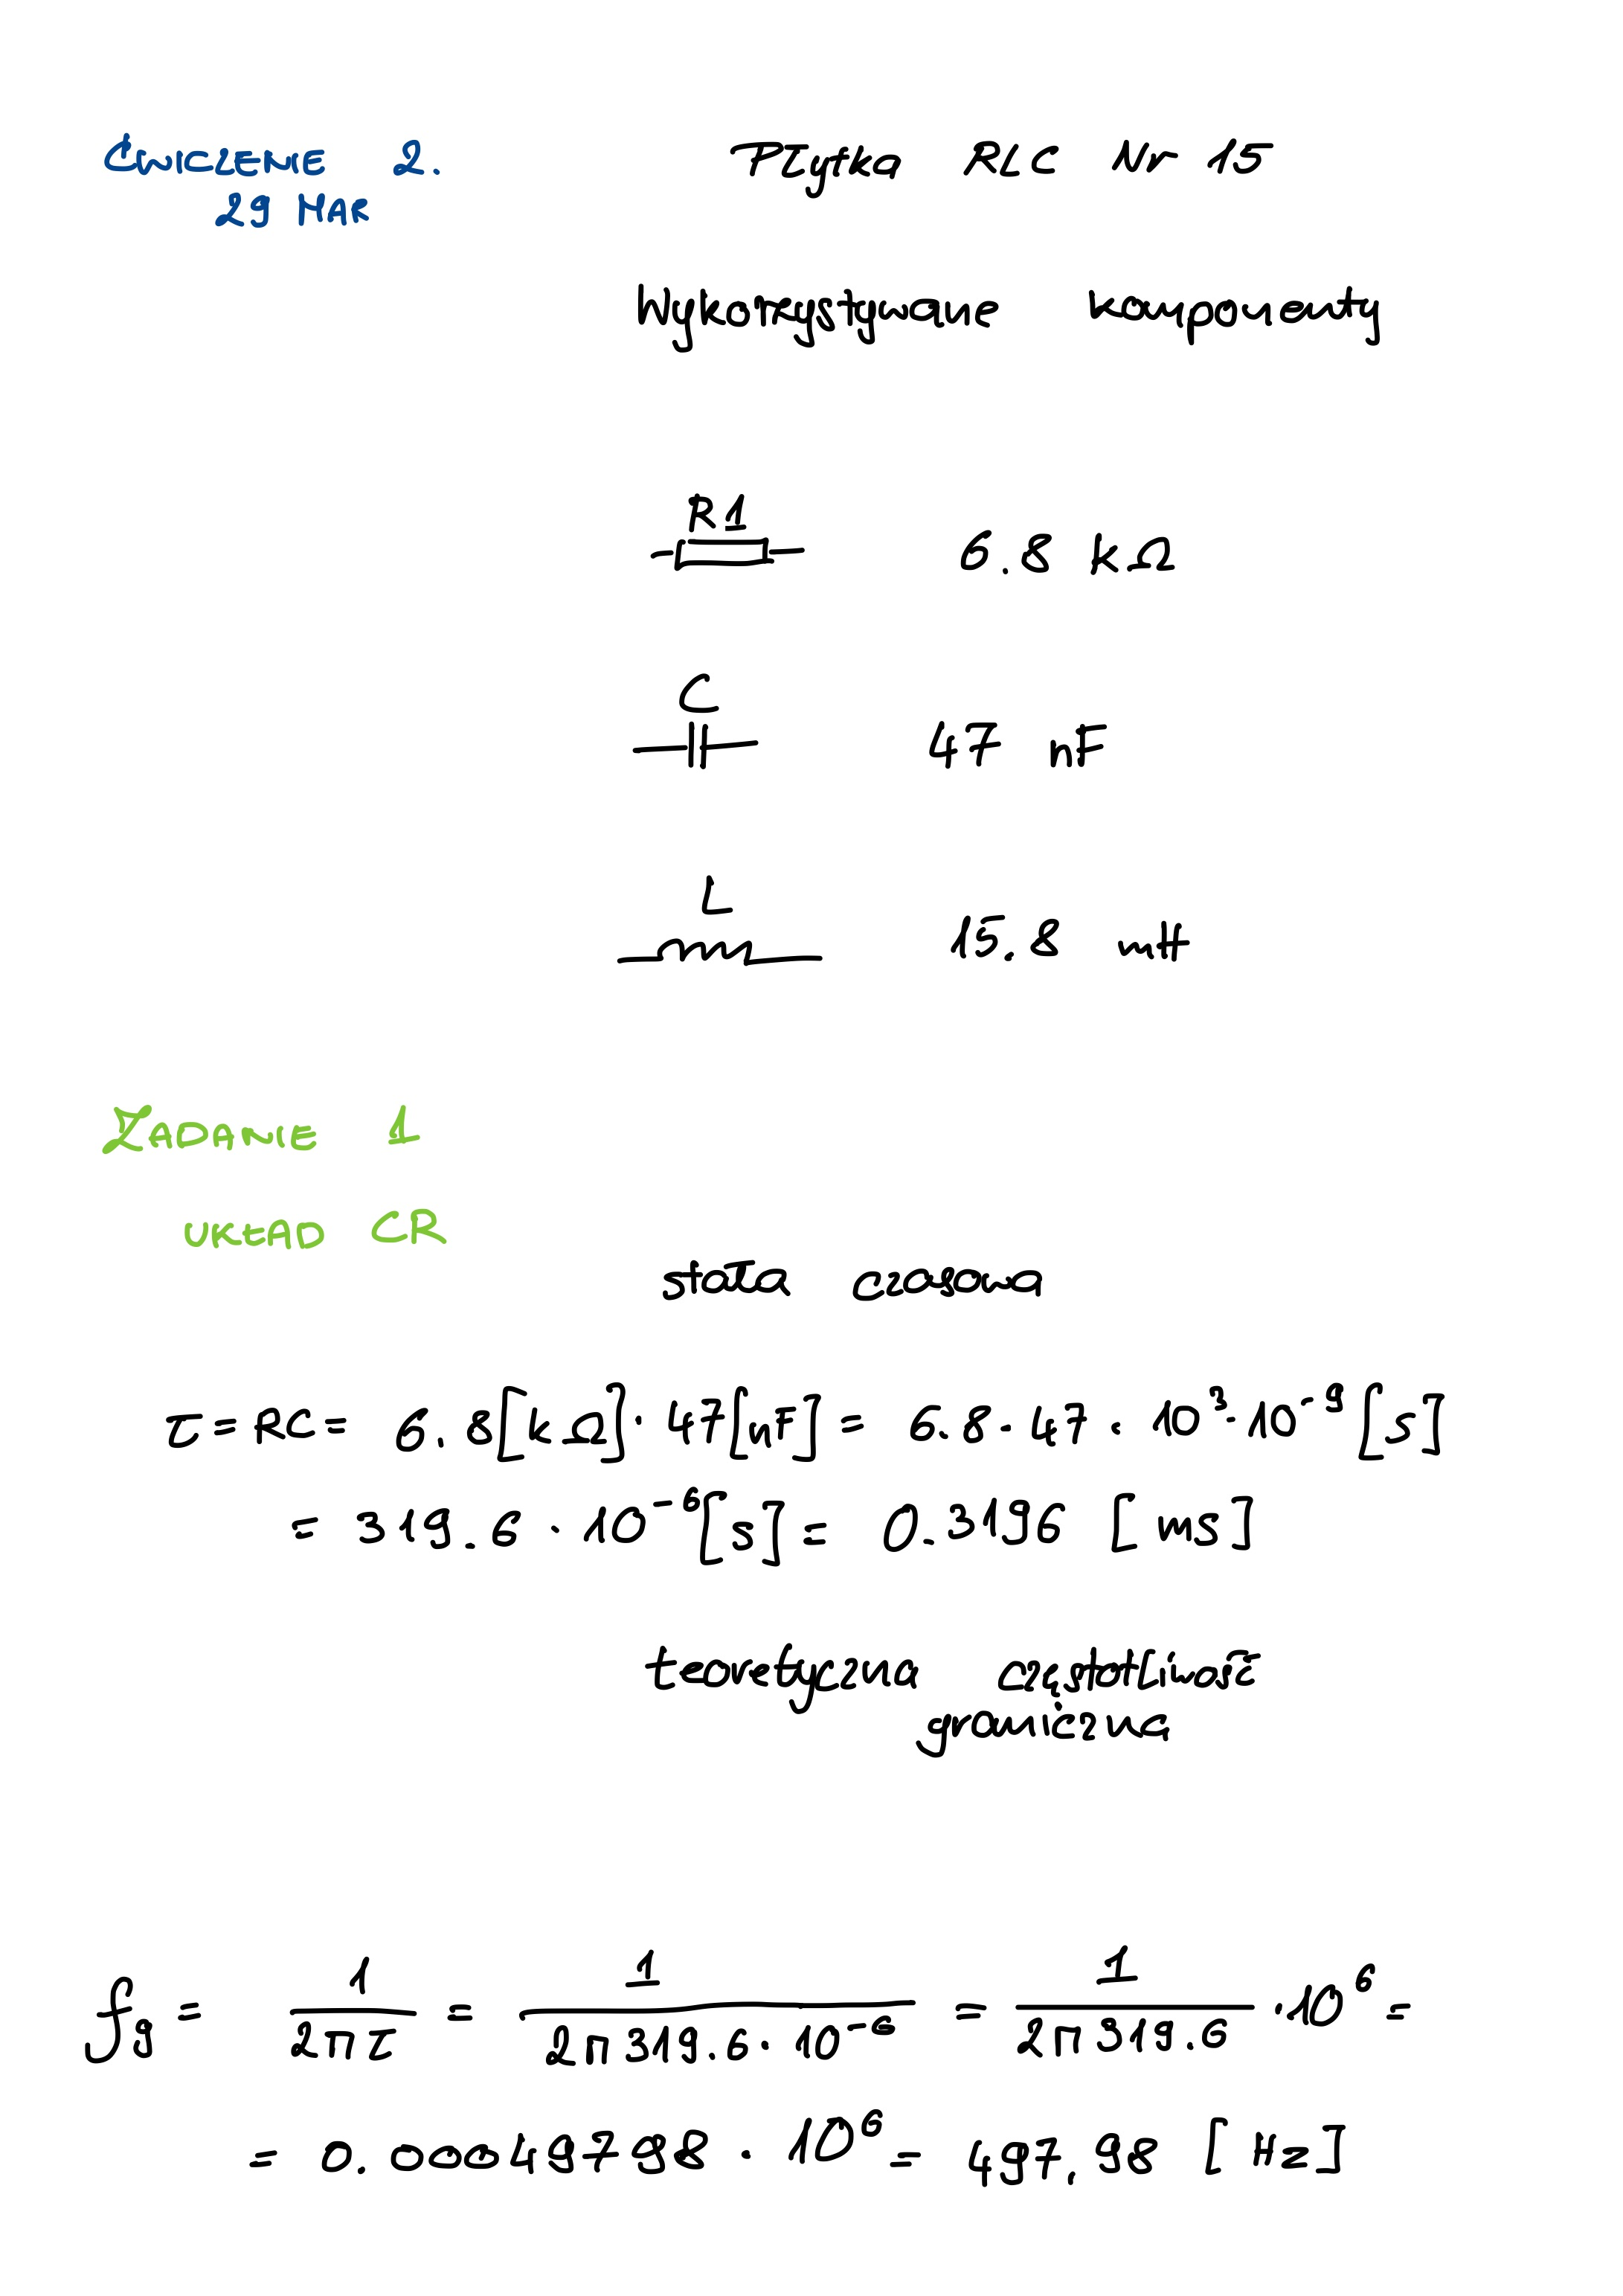
\includegraphics[scale=0.2]{B0}
\centering
\captionsetup{labelformat=empty}
\caption{}
\end{figure}

\begin{figure}[H]
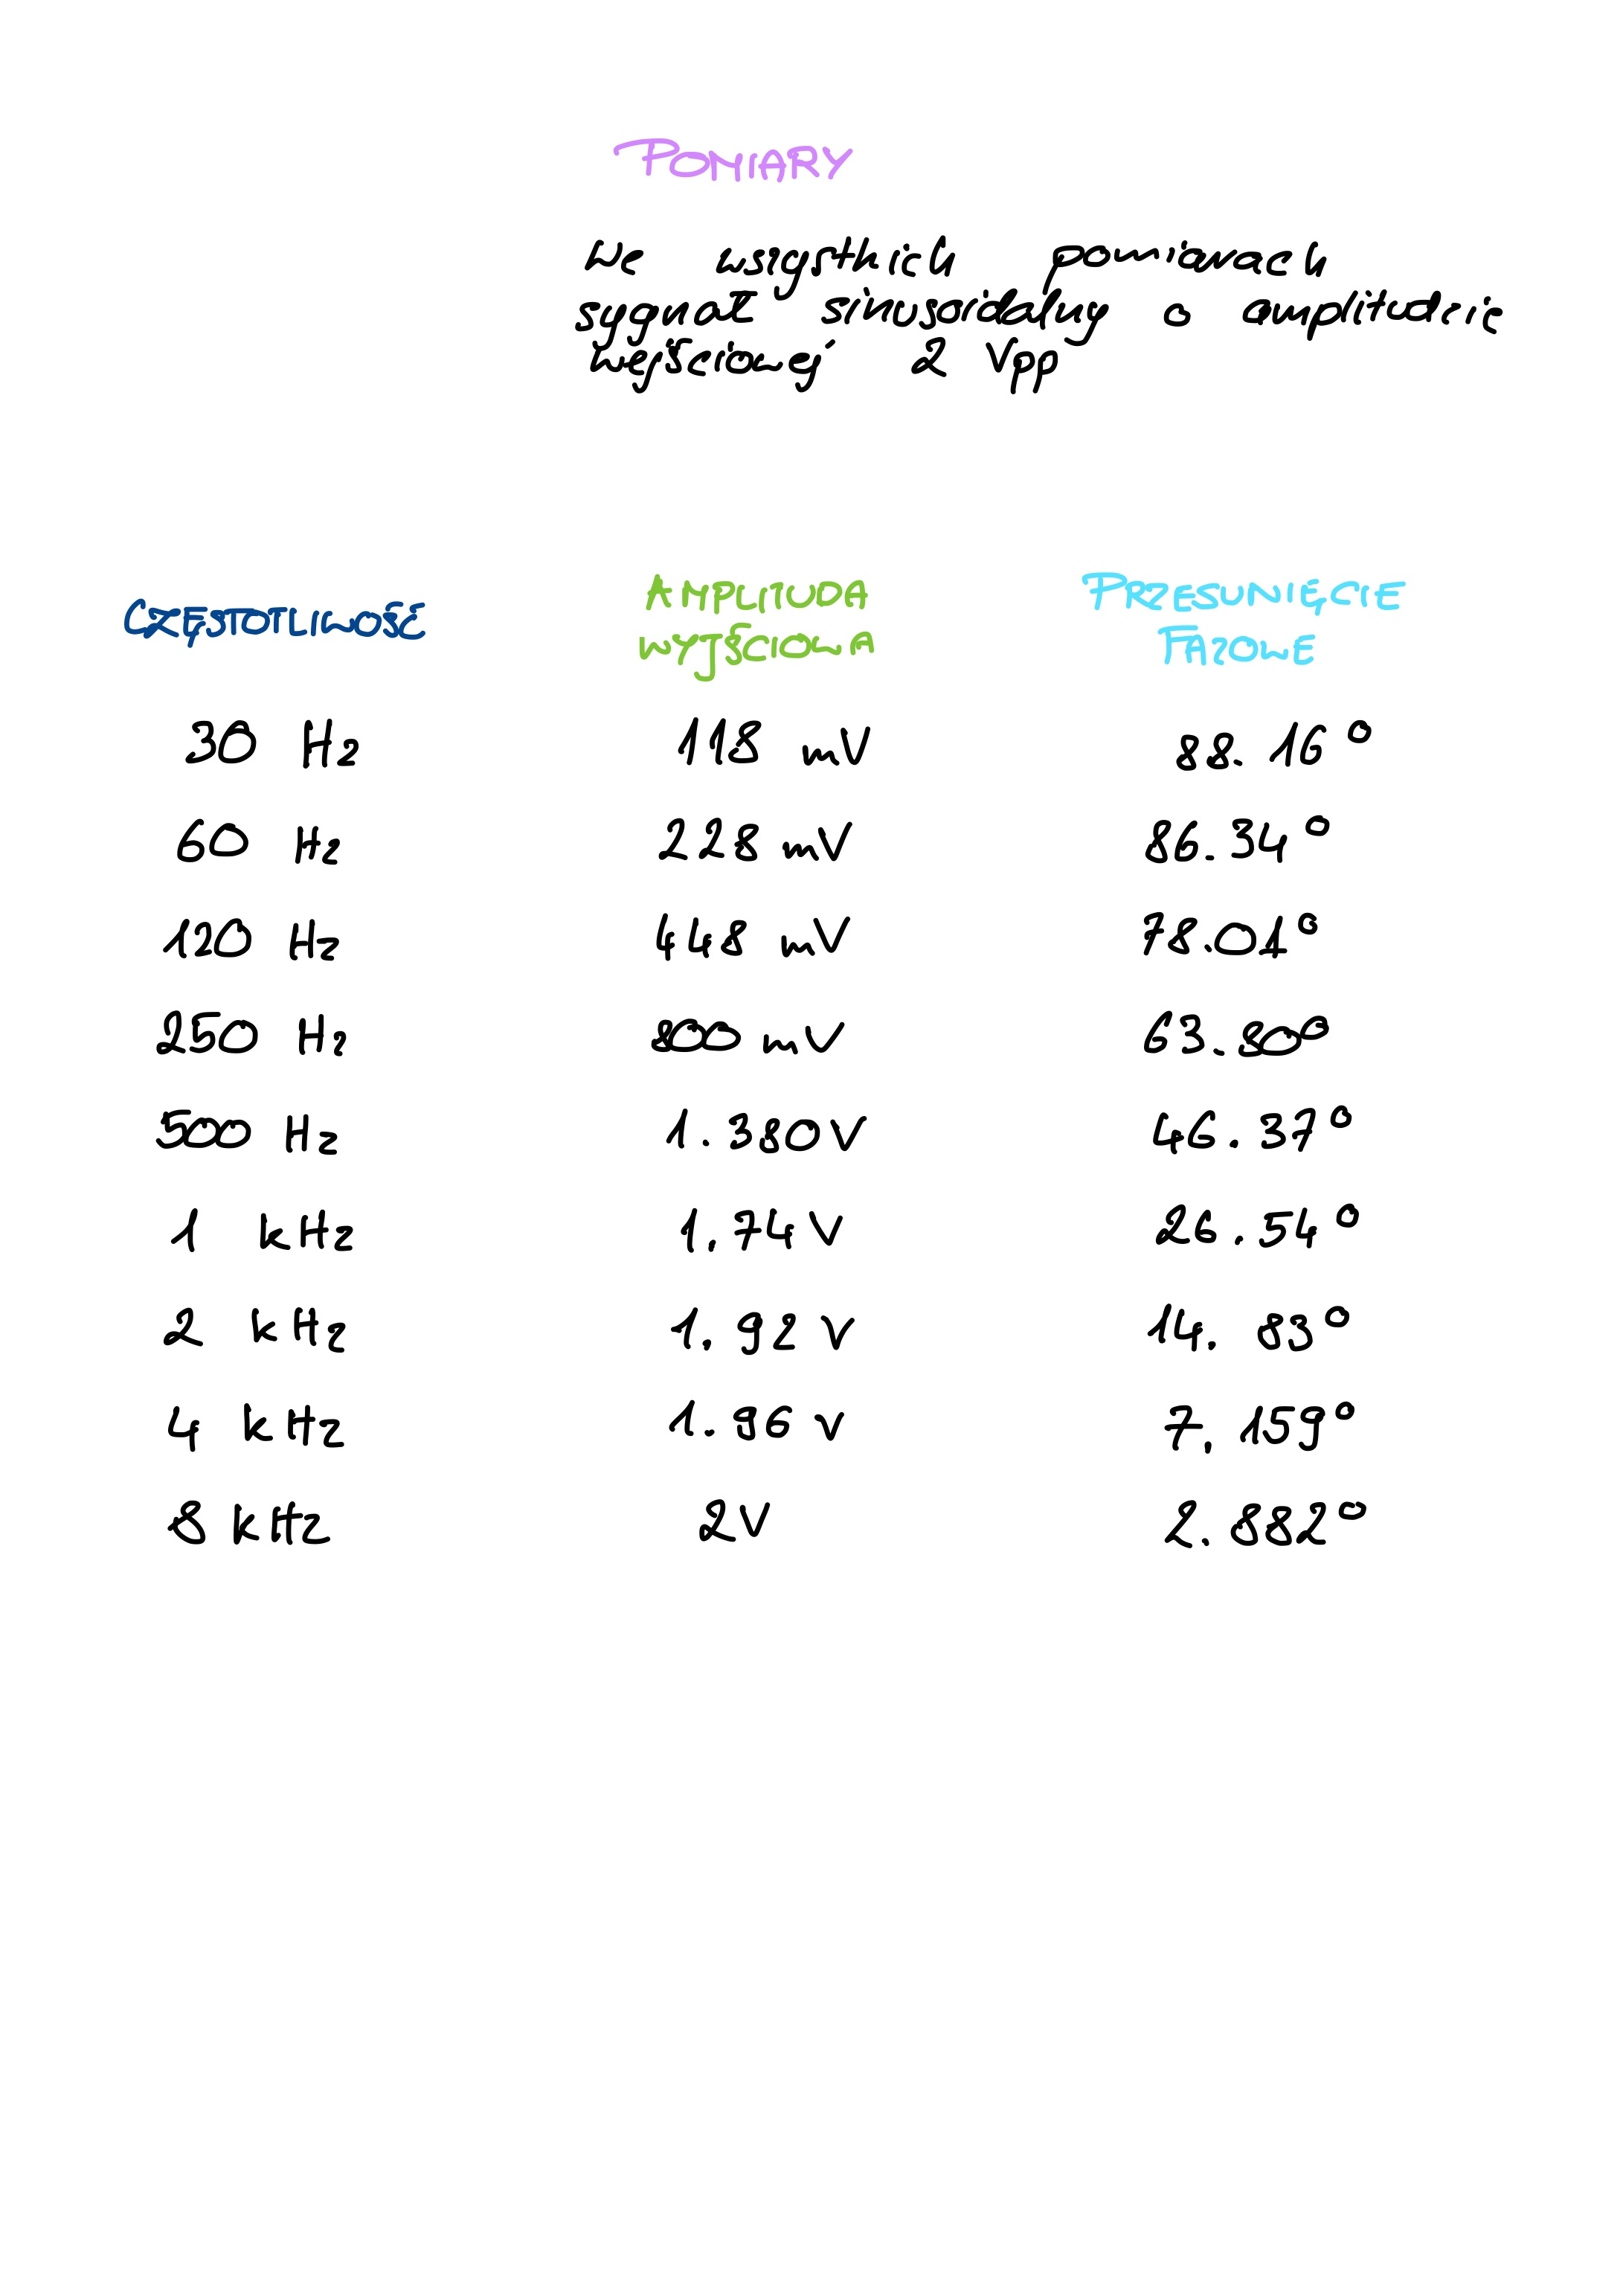
\includegraphics[scale=0.2]{B1}
\centering
\captionsetup{labelformat=empty}
\caption{}
\end{figure}

\begin{figure}[H]
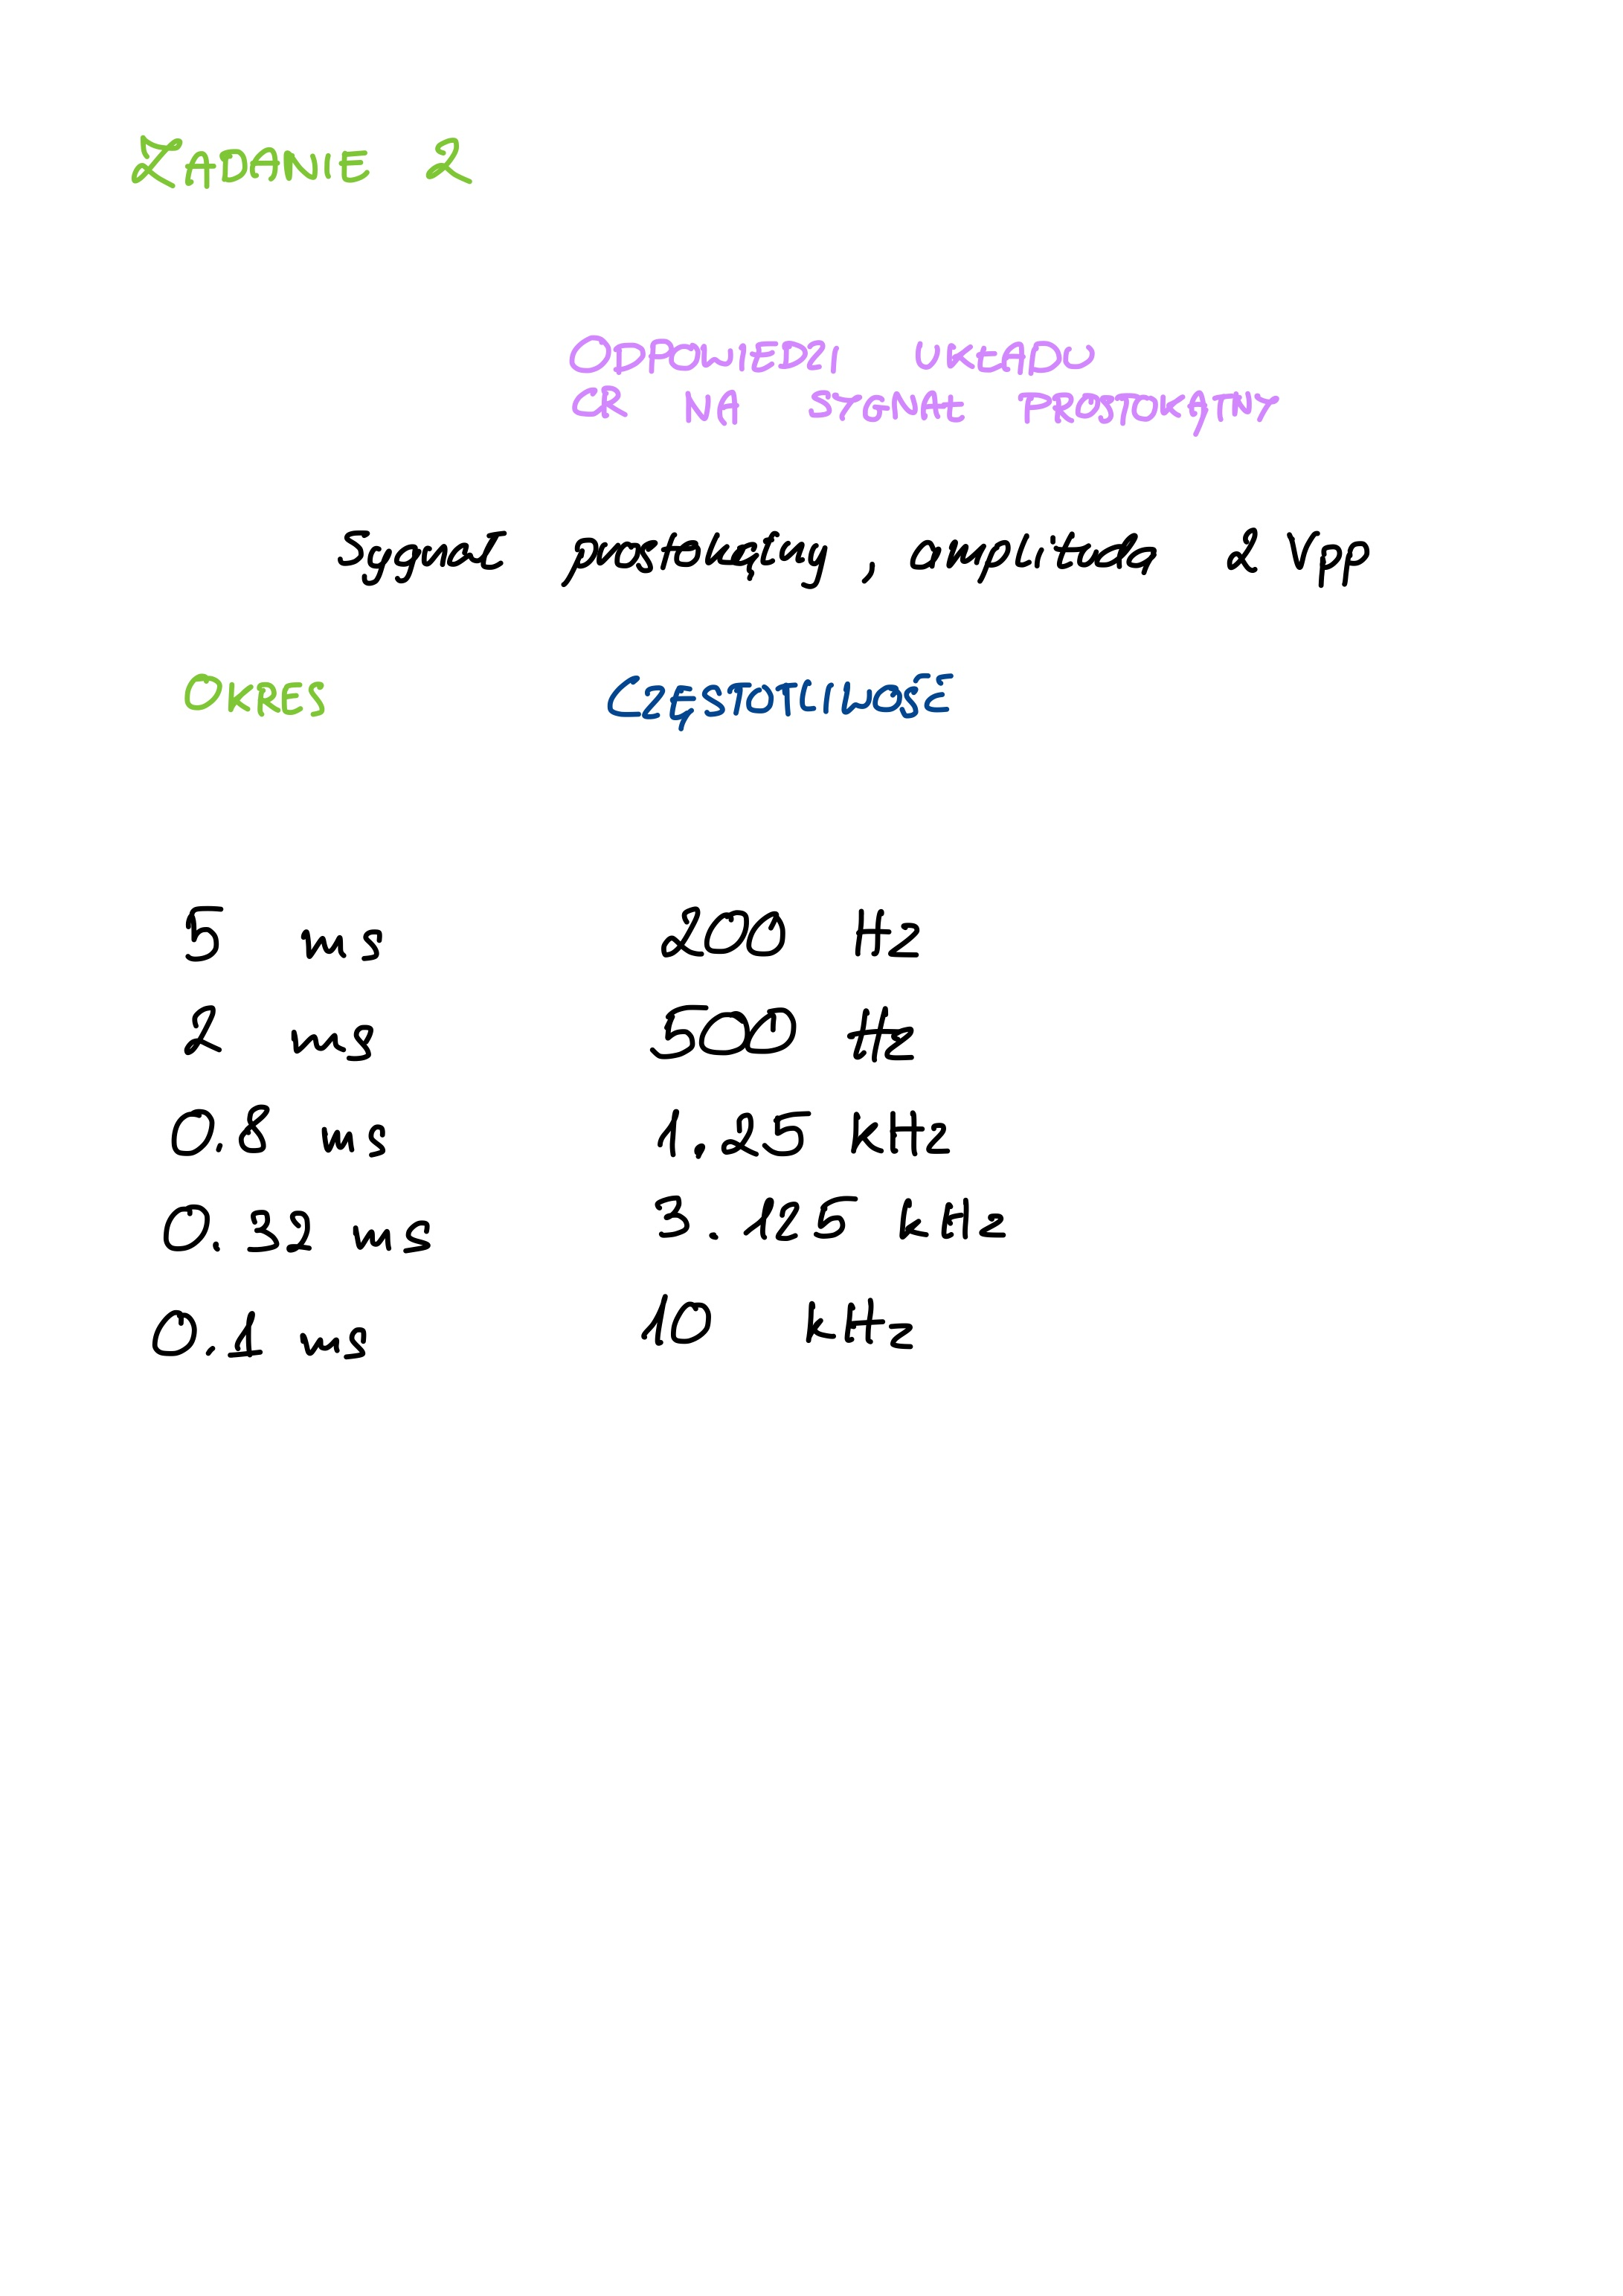
\includegraphics[scale=0.2]{B2}
\centering
\captionsetup{labelformat=empty}
\caption{}
\end{figure}

\begin{figure}[H]
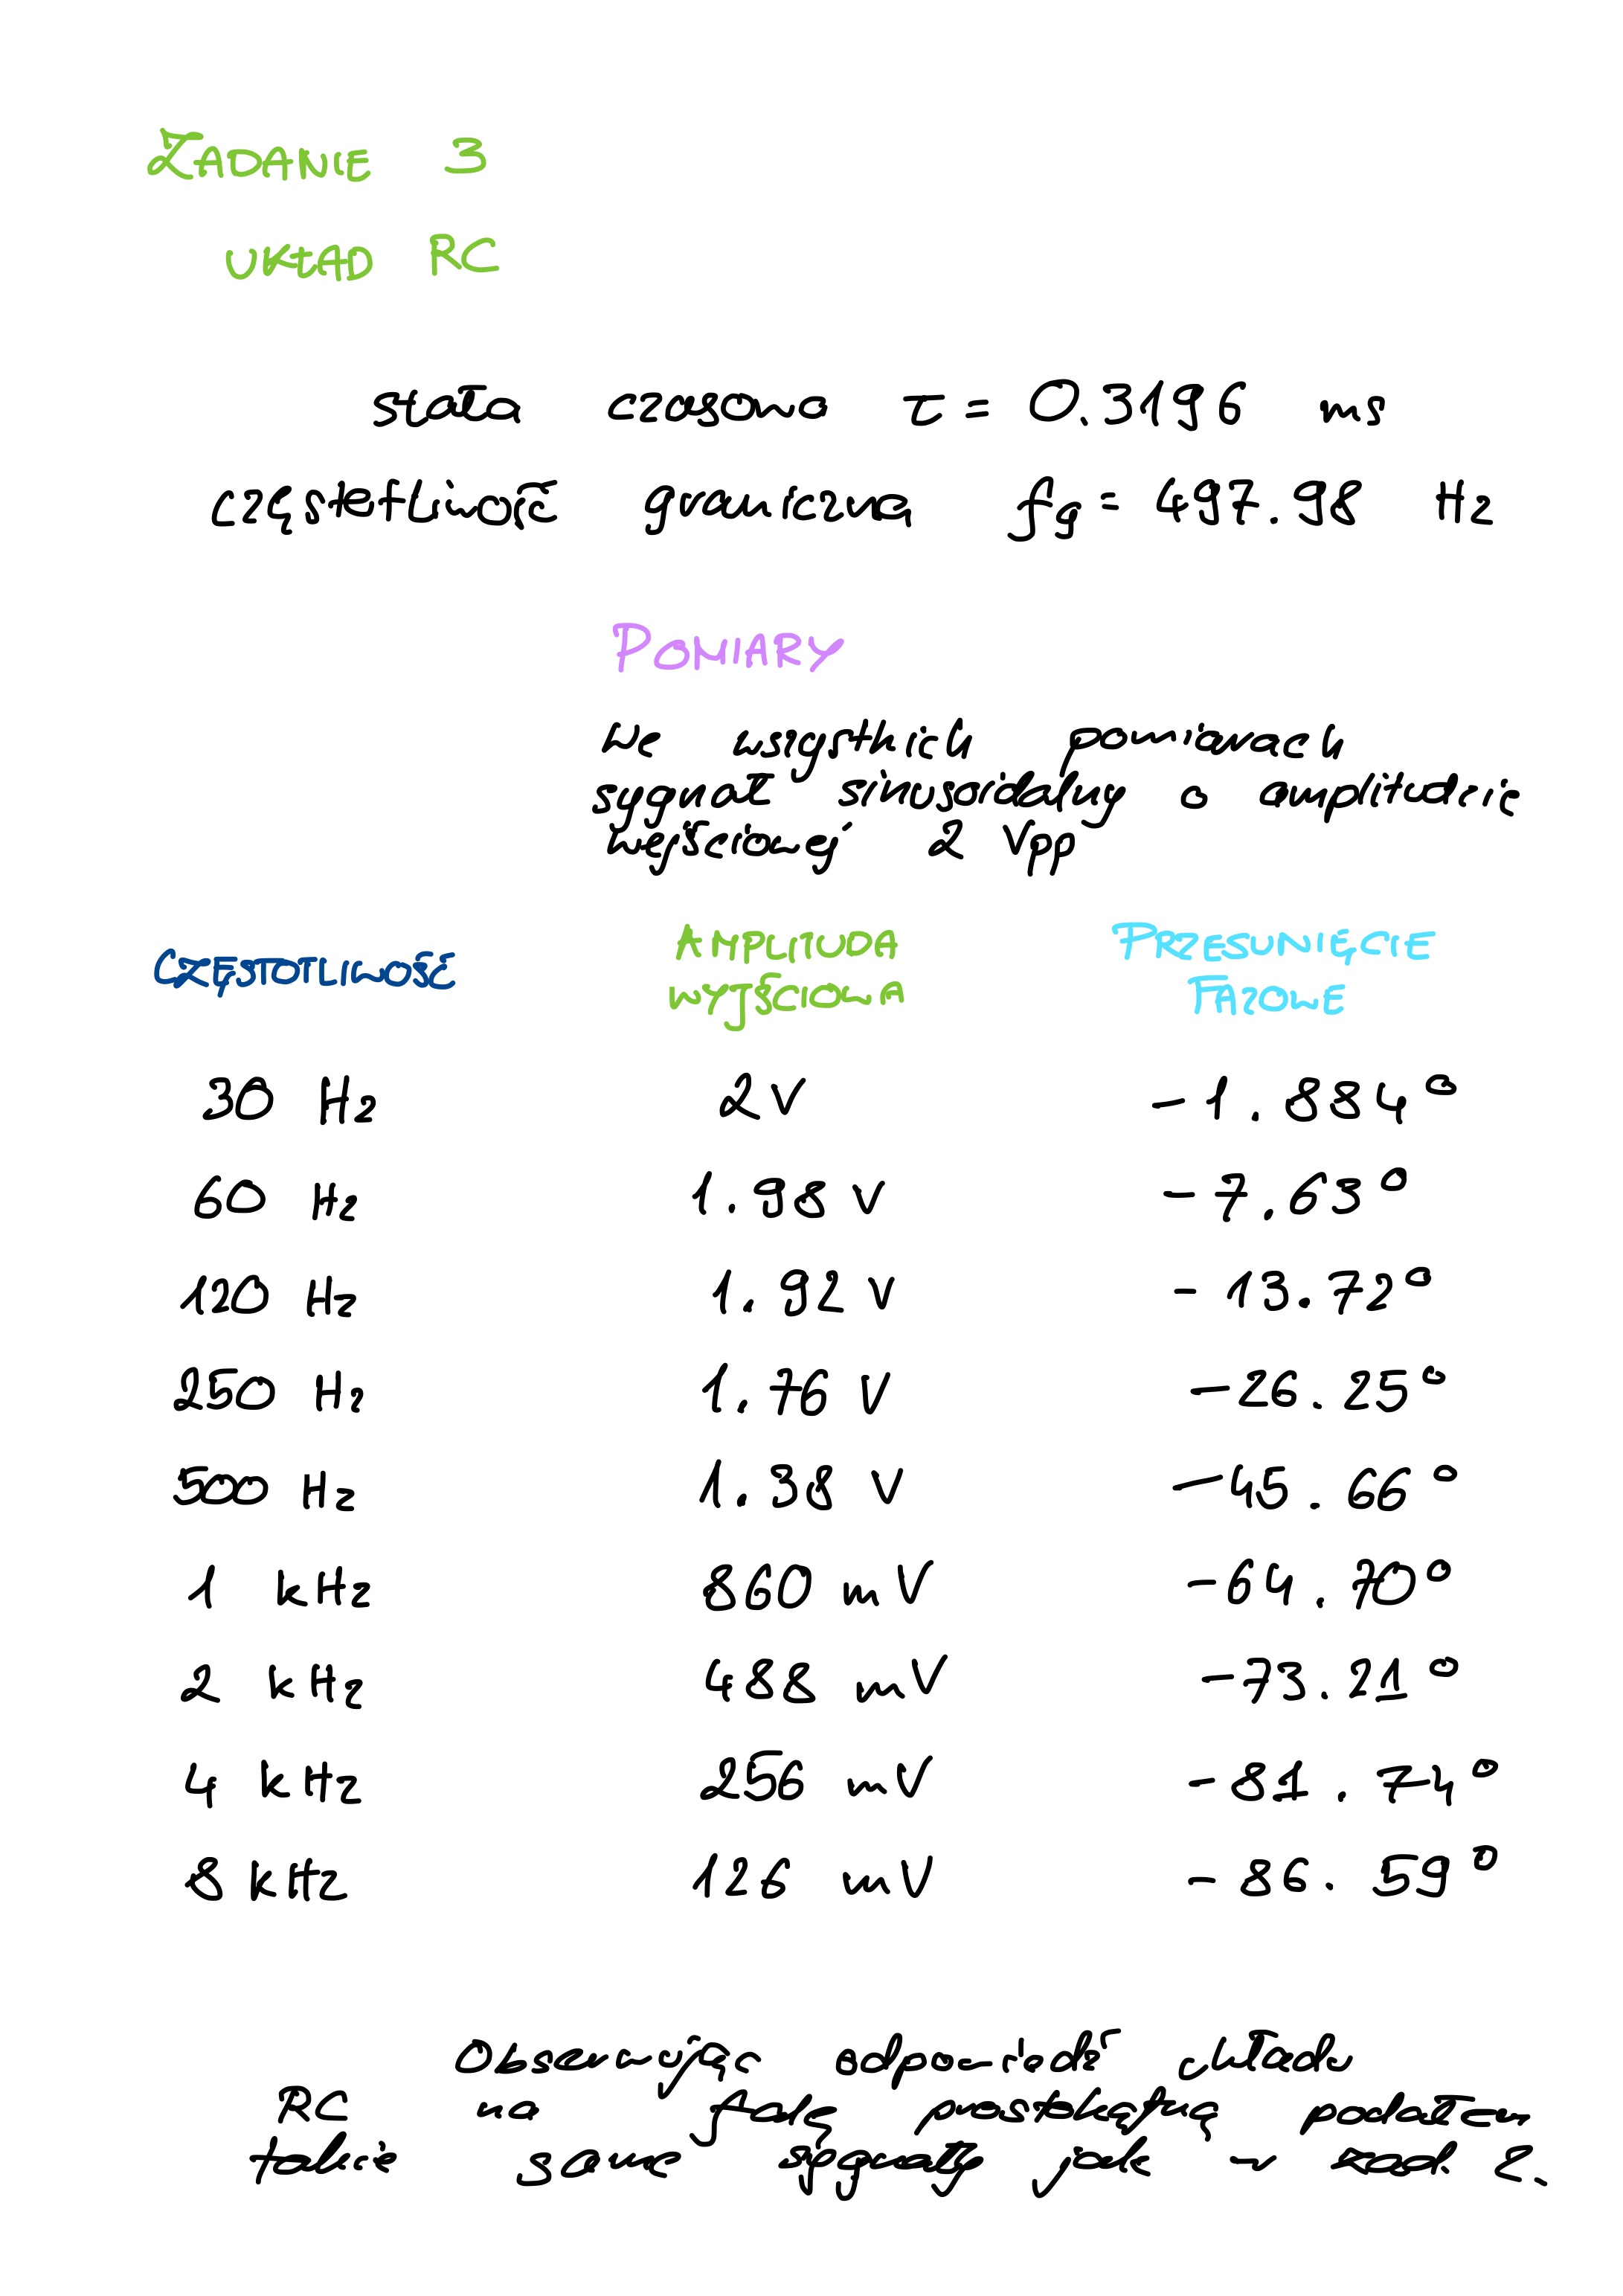
\includegraphics[scale=0.2]{B3}
\centering
\captionsetup{labelformat=empty}
\caption{}
\end{figure}

\begin{figure}[H]
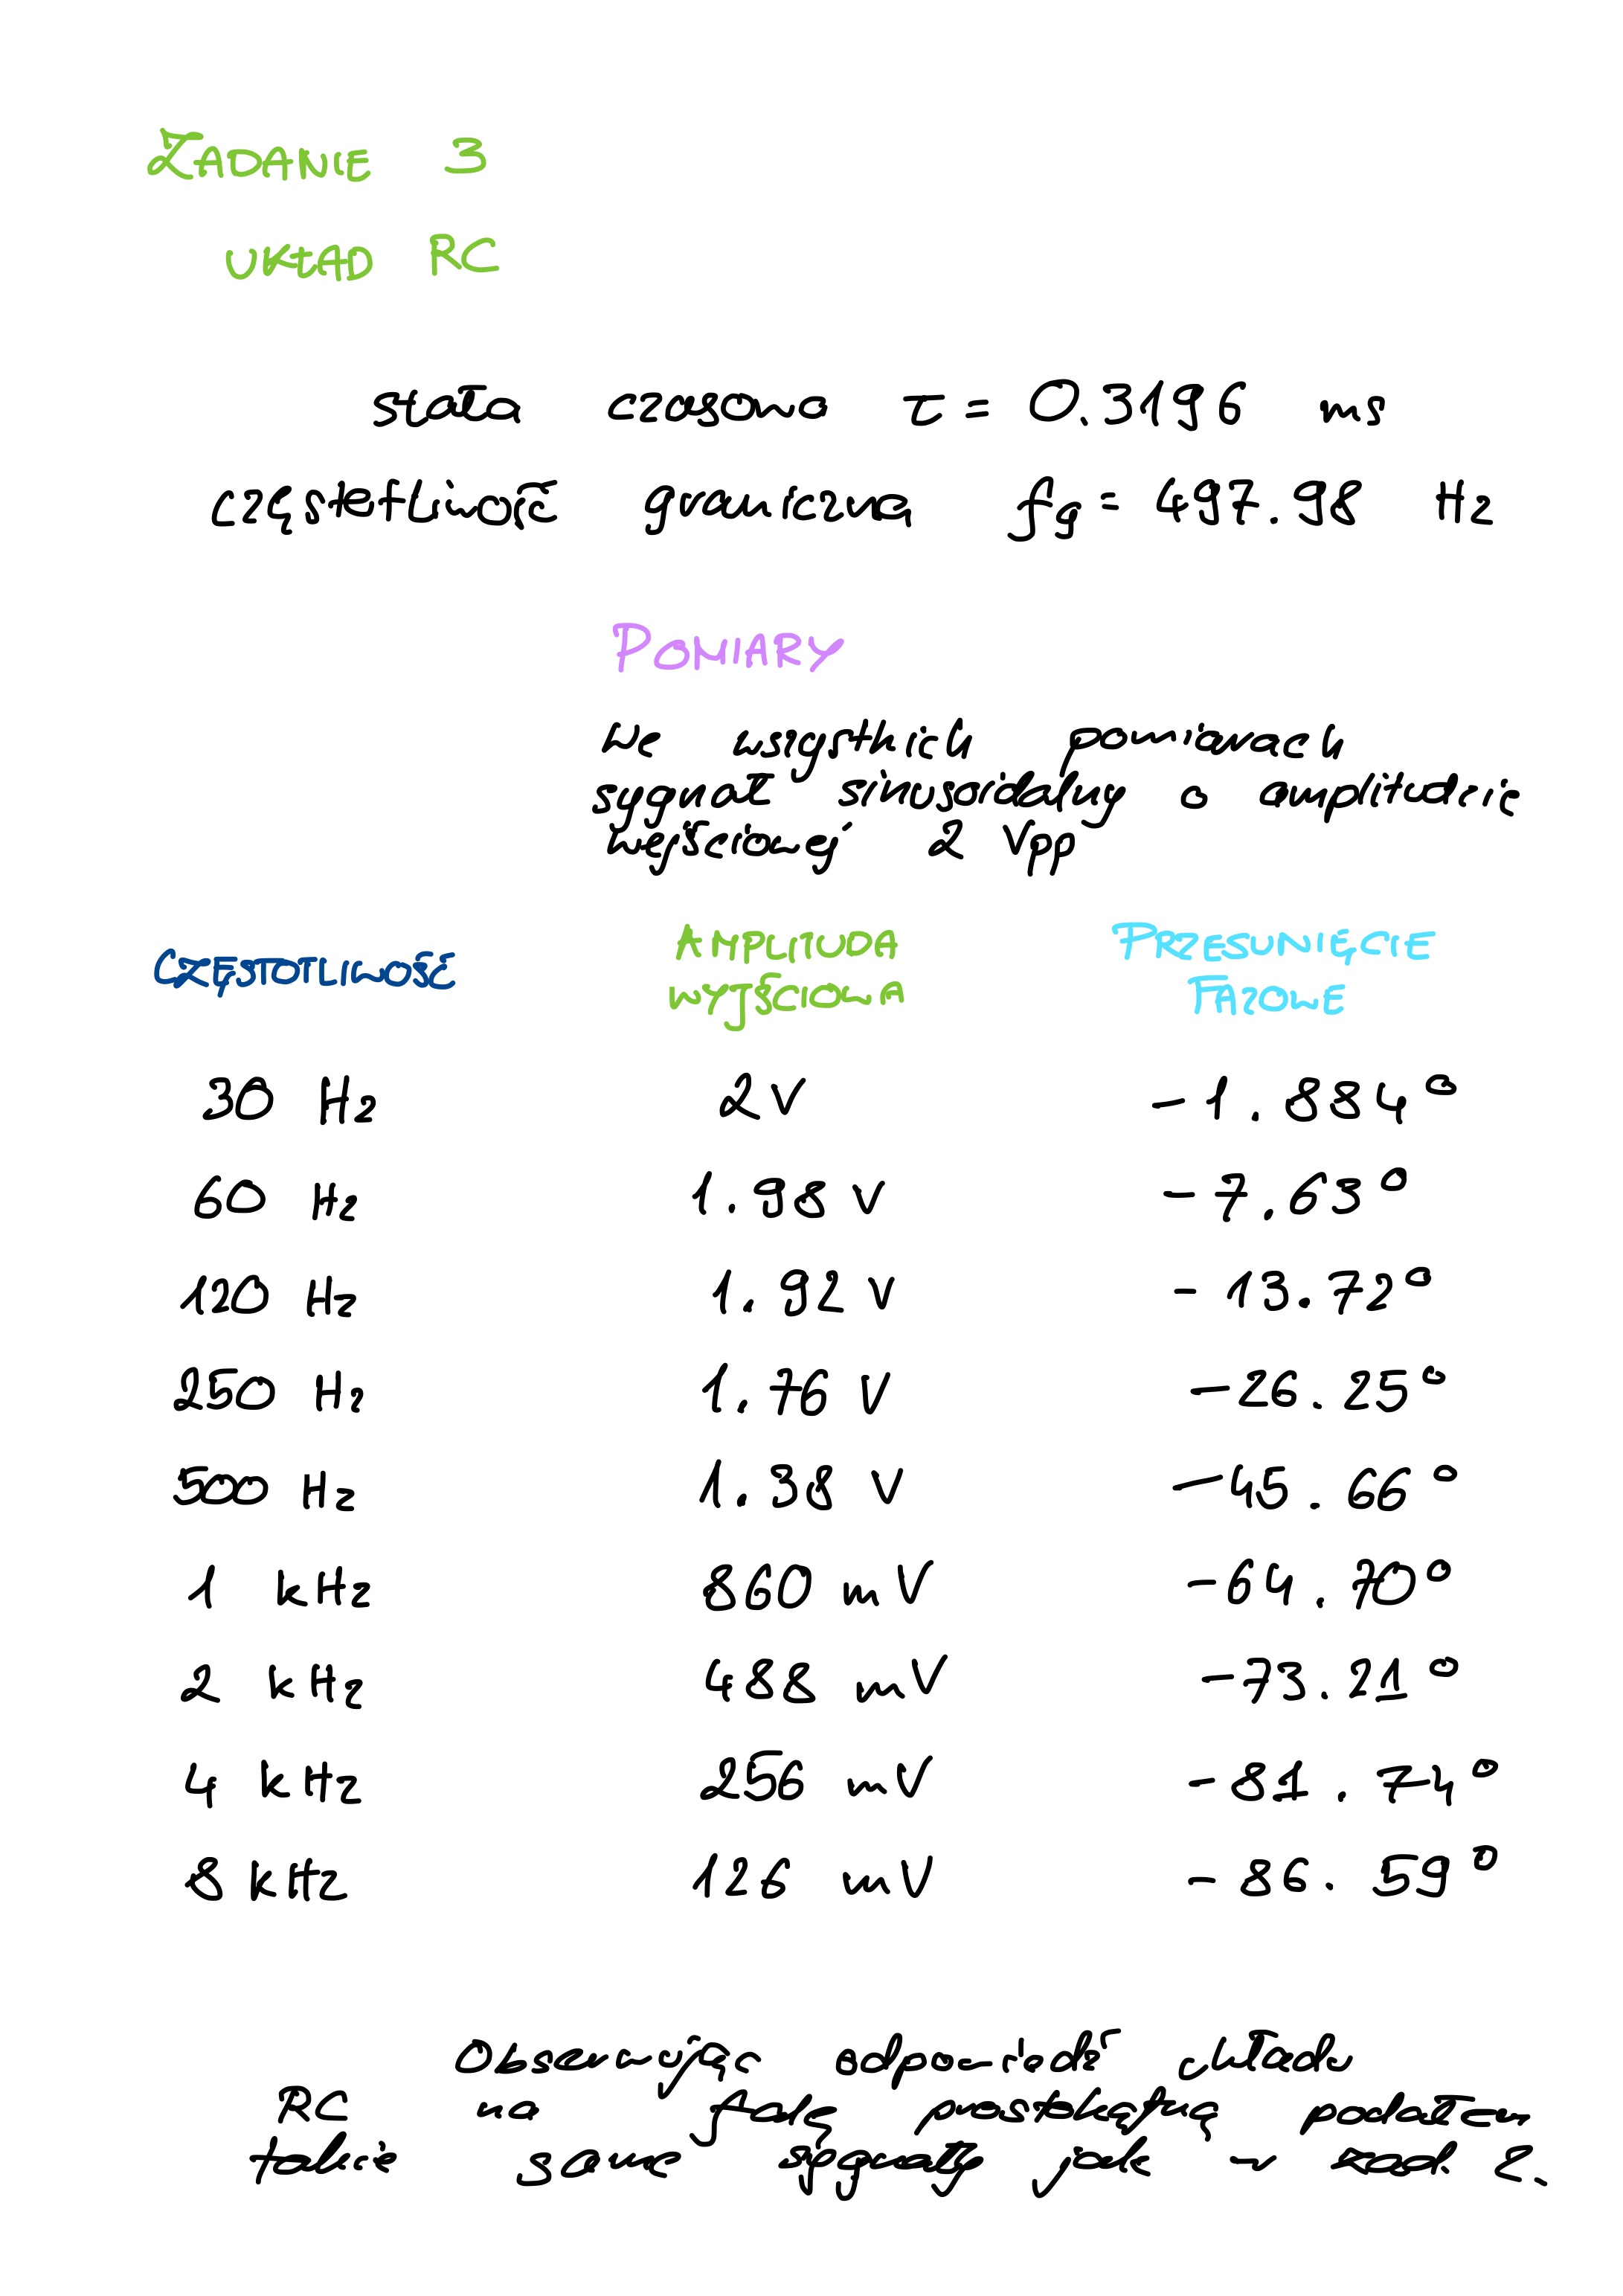
\includegraphics[scale=0.2]{B3}
\centering
\captionsetup{labelformat=empty}
\caption{}
\end{figure}

\end{document}